%	e-Yantra, IIT-Bombay

%	Document Author: Chinmay Patil
%	Date: 11-July,2016
%	Last Edited by: Chinmay
%   Date Last updated: 11-06-2016 

%%%%%%%%%%%%%%%%%%%%%%%%%%%%%%%%%%%%%%%%%%%%%%%%%%%%%%%%%%%%%%%%%%%%%%%%%%%%%


\documentclass[11pt,a4paper]{article}
\usepackage{graphicx}
\usepackage{listings}
\usepackage{graphics}
\usepackage{wrapfig}
\usepackage[T1]{fontenc}
\usepackage[margin=1.2in]{geometry}
\usepackage{tcolorbox}
\usepackage{hyperref}
\usepackage{dingbat}
\usepackage{float}
\usepackage{tocloft}

\begin{document}
\begin{titlepage}
\title{Manual for running wiced sense}
\author{e-Yantra Team}
\date{\today}
\maketitle
\end{titlepage}

\tableofcontents
    \newpage
	\section{How to use wiced sense GUI ?}
	\subsection{Sensor Data display Page}
	
	 \begin{itemize}
	 \item Open terminal and start lampp local server.
	 
	 	\begin{figure}[h]
    \centering
	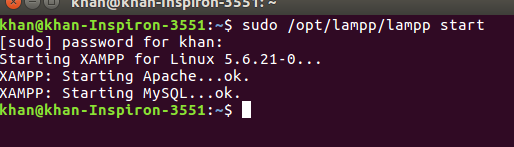
\includegraphics[scale=0.5]{lampstart.png}
	\end{figure}
	 
	 \item Open Sensor.html page in website.
	 \item Insert USB (zigbee) into the USB slot of local machine.
	 
	 \begin{figure}[h]
        \centering
	    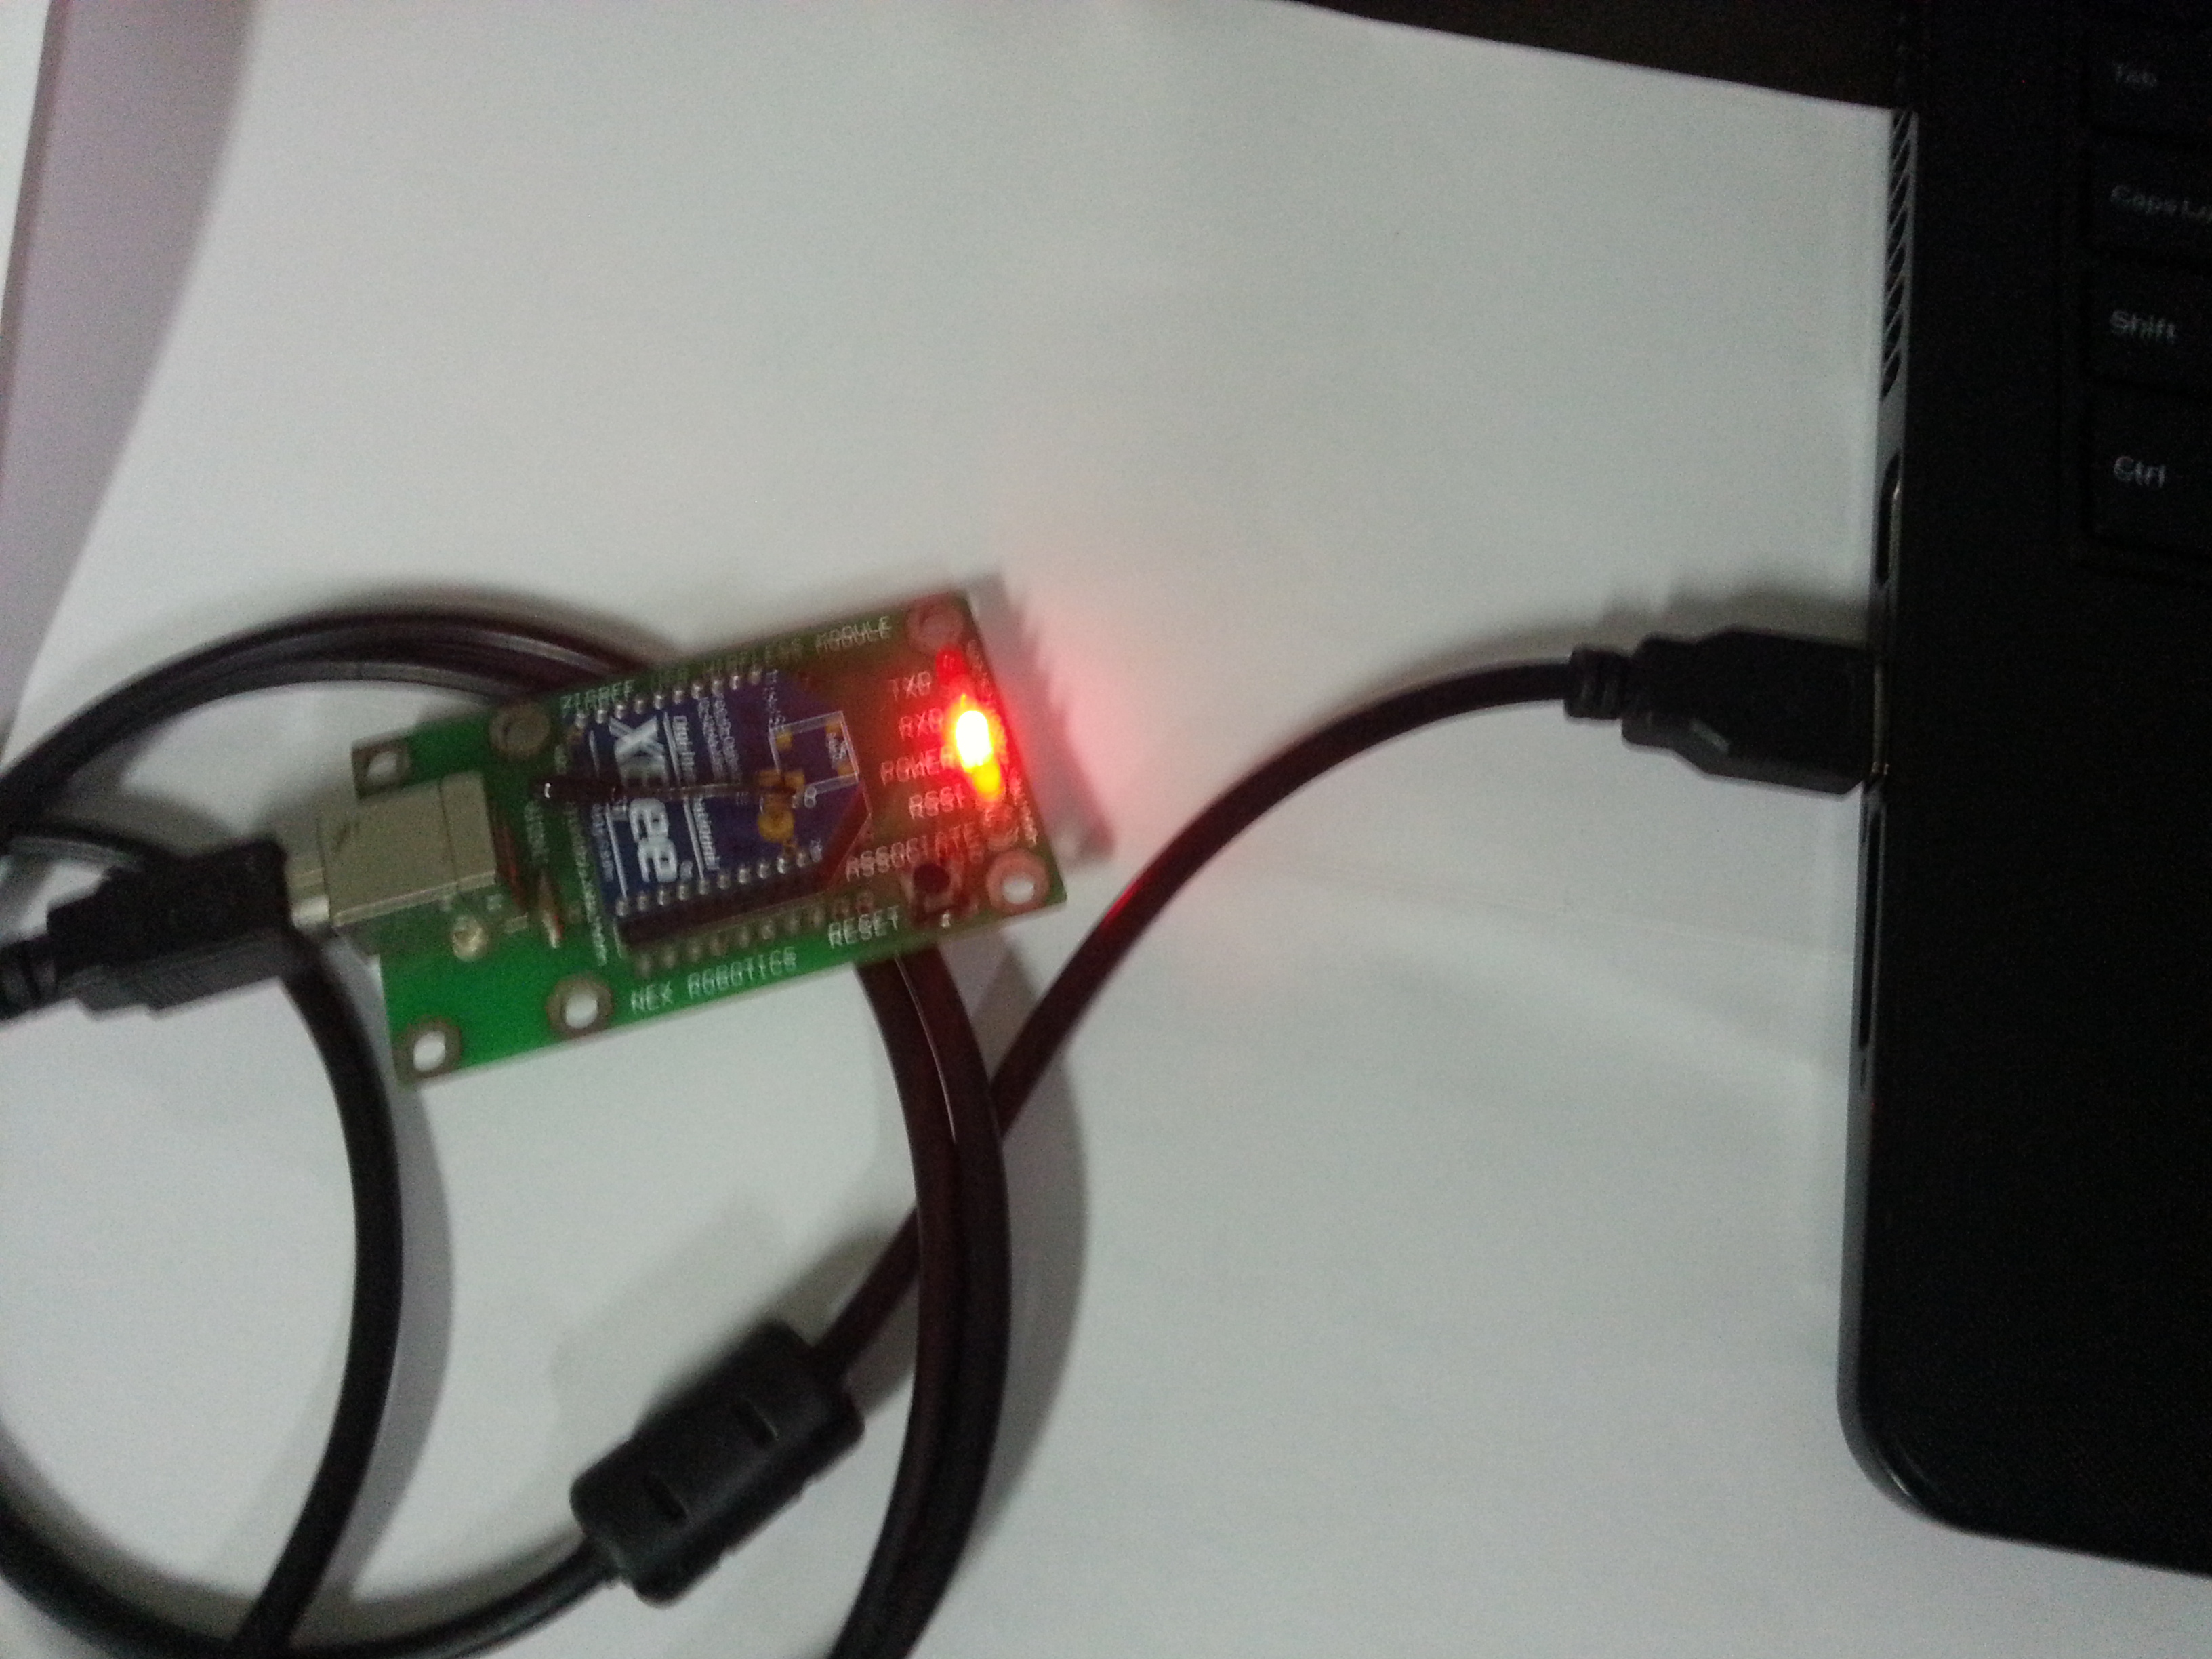
\includegraphics[scale=0.1]{20160722_194935.jpg}
	\end{figure}
	 
	 \item Turn ON bluetooth and run wiced.js file in terminal
	 
	 \begin{figure}[h]
    \centering
	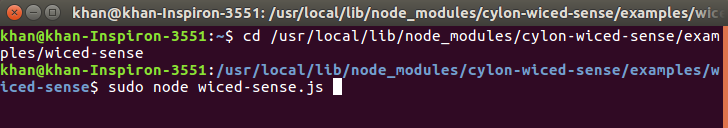
\includegraphics[scale=0.5]{runwicedjs.png}
	\end{figure}

	 \item As data arrives on terminal the data will be displayed on the page.
	 
	 \newpage 
	 \item Compass and acceleration reading will be displayed immediately according to the sensor data. But data of humidity, temperature, pressure are displayed after some delay of 2-3 sec.
	 
	 \begin{figure}[h]
    \centering
	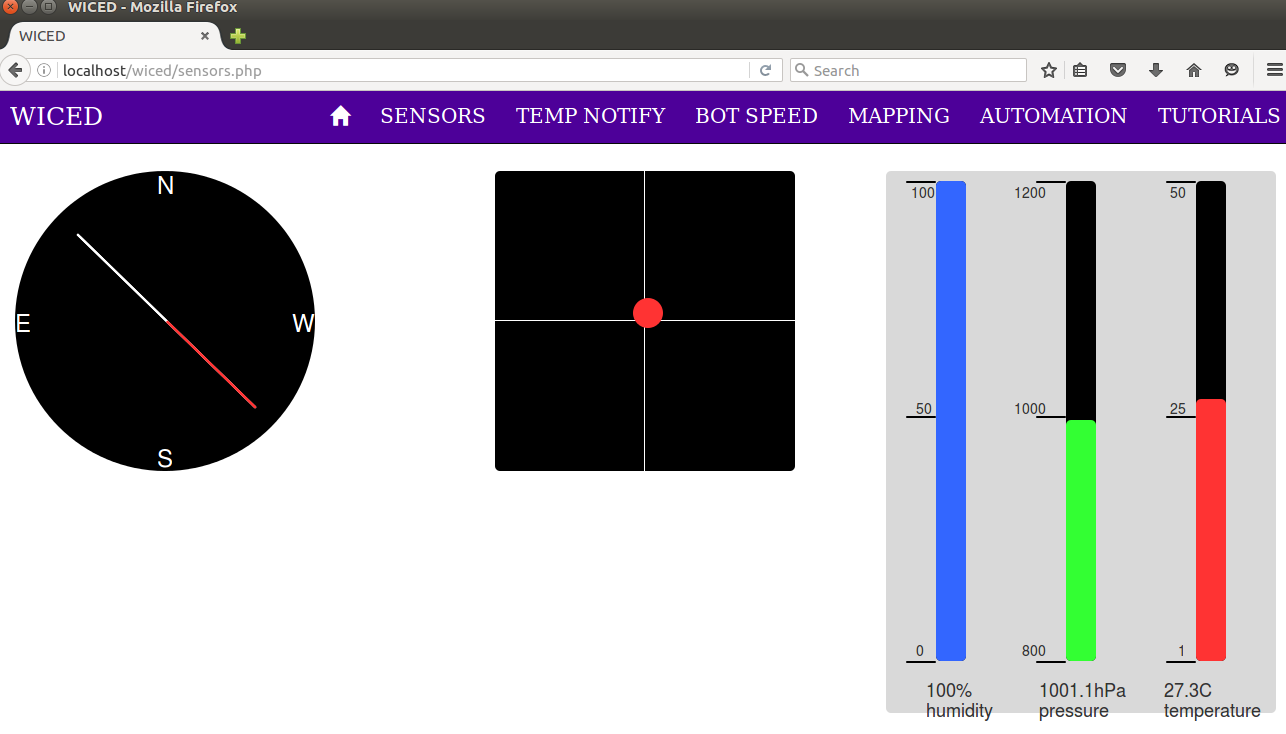
\includegraphics[scale=0.3]{sensor.png}
	\end{figure}
	 \end{itemize}
	 
	 
	 
	 \newpage
	 \subsection{How to use temperature notifier ?}
	 
	 \begin{itemize}
	 \item Open terminal and start lampp local server.
	 
	 	\begin{figure}[h]
    \centering
	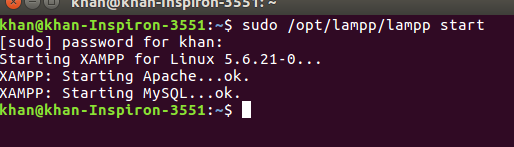
\includegraphics[scale=0.5]{lampstart.png}
	\end{figure}
	 
	 \item Open temp.html page in website.
	 \item Insert USB (zigbee) into the USB slot of local machine.
	 
	 \begin{figure}[h]
        \centering
	    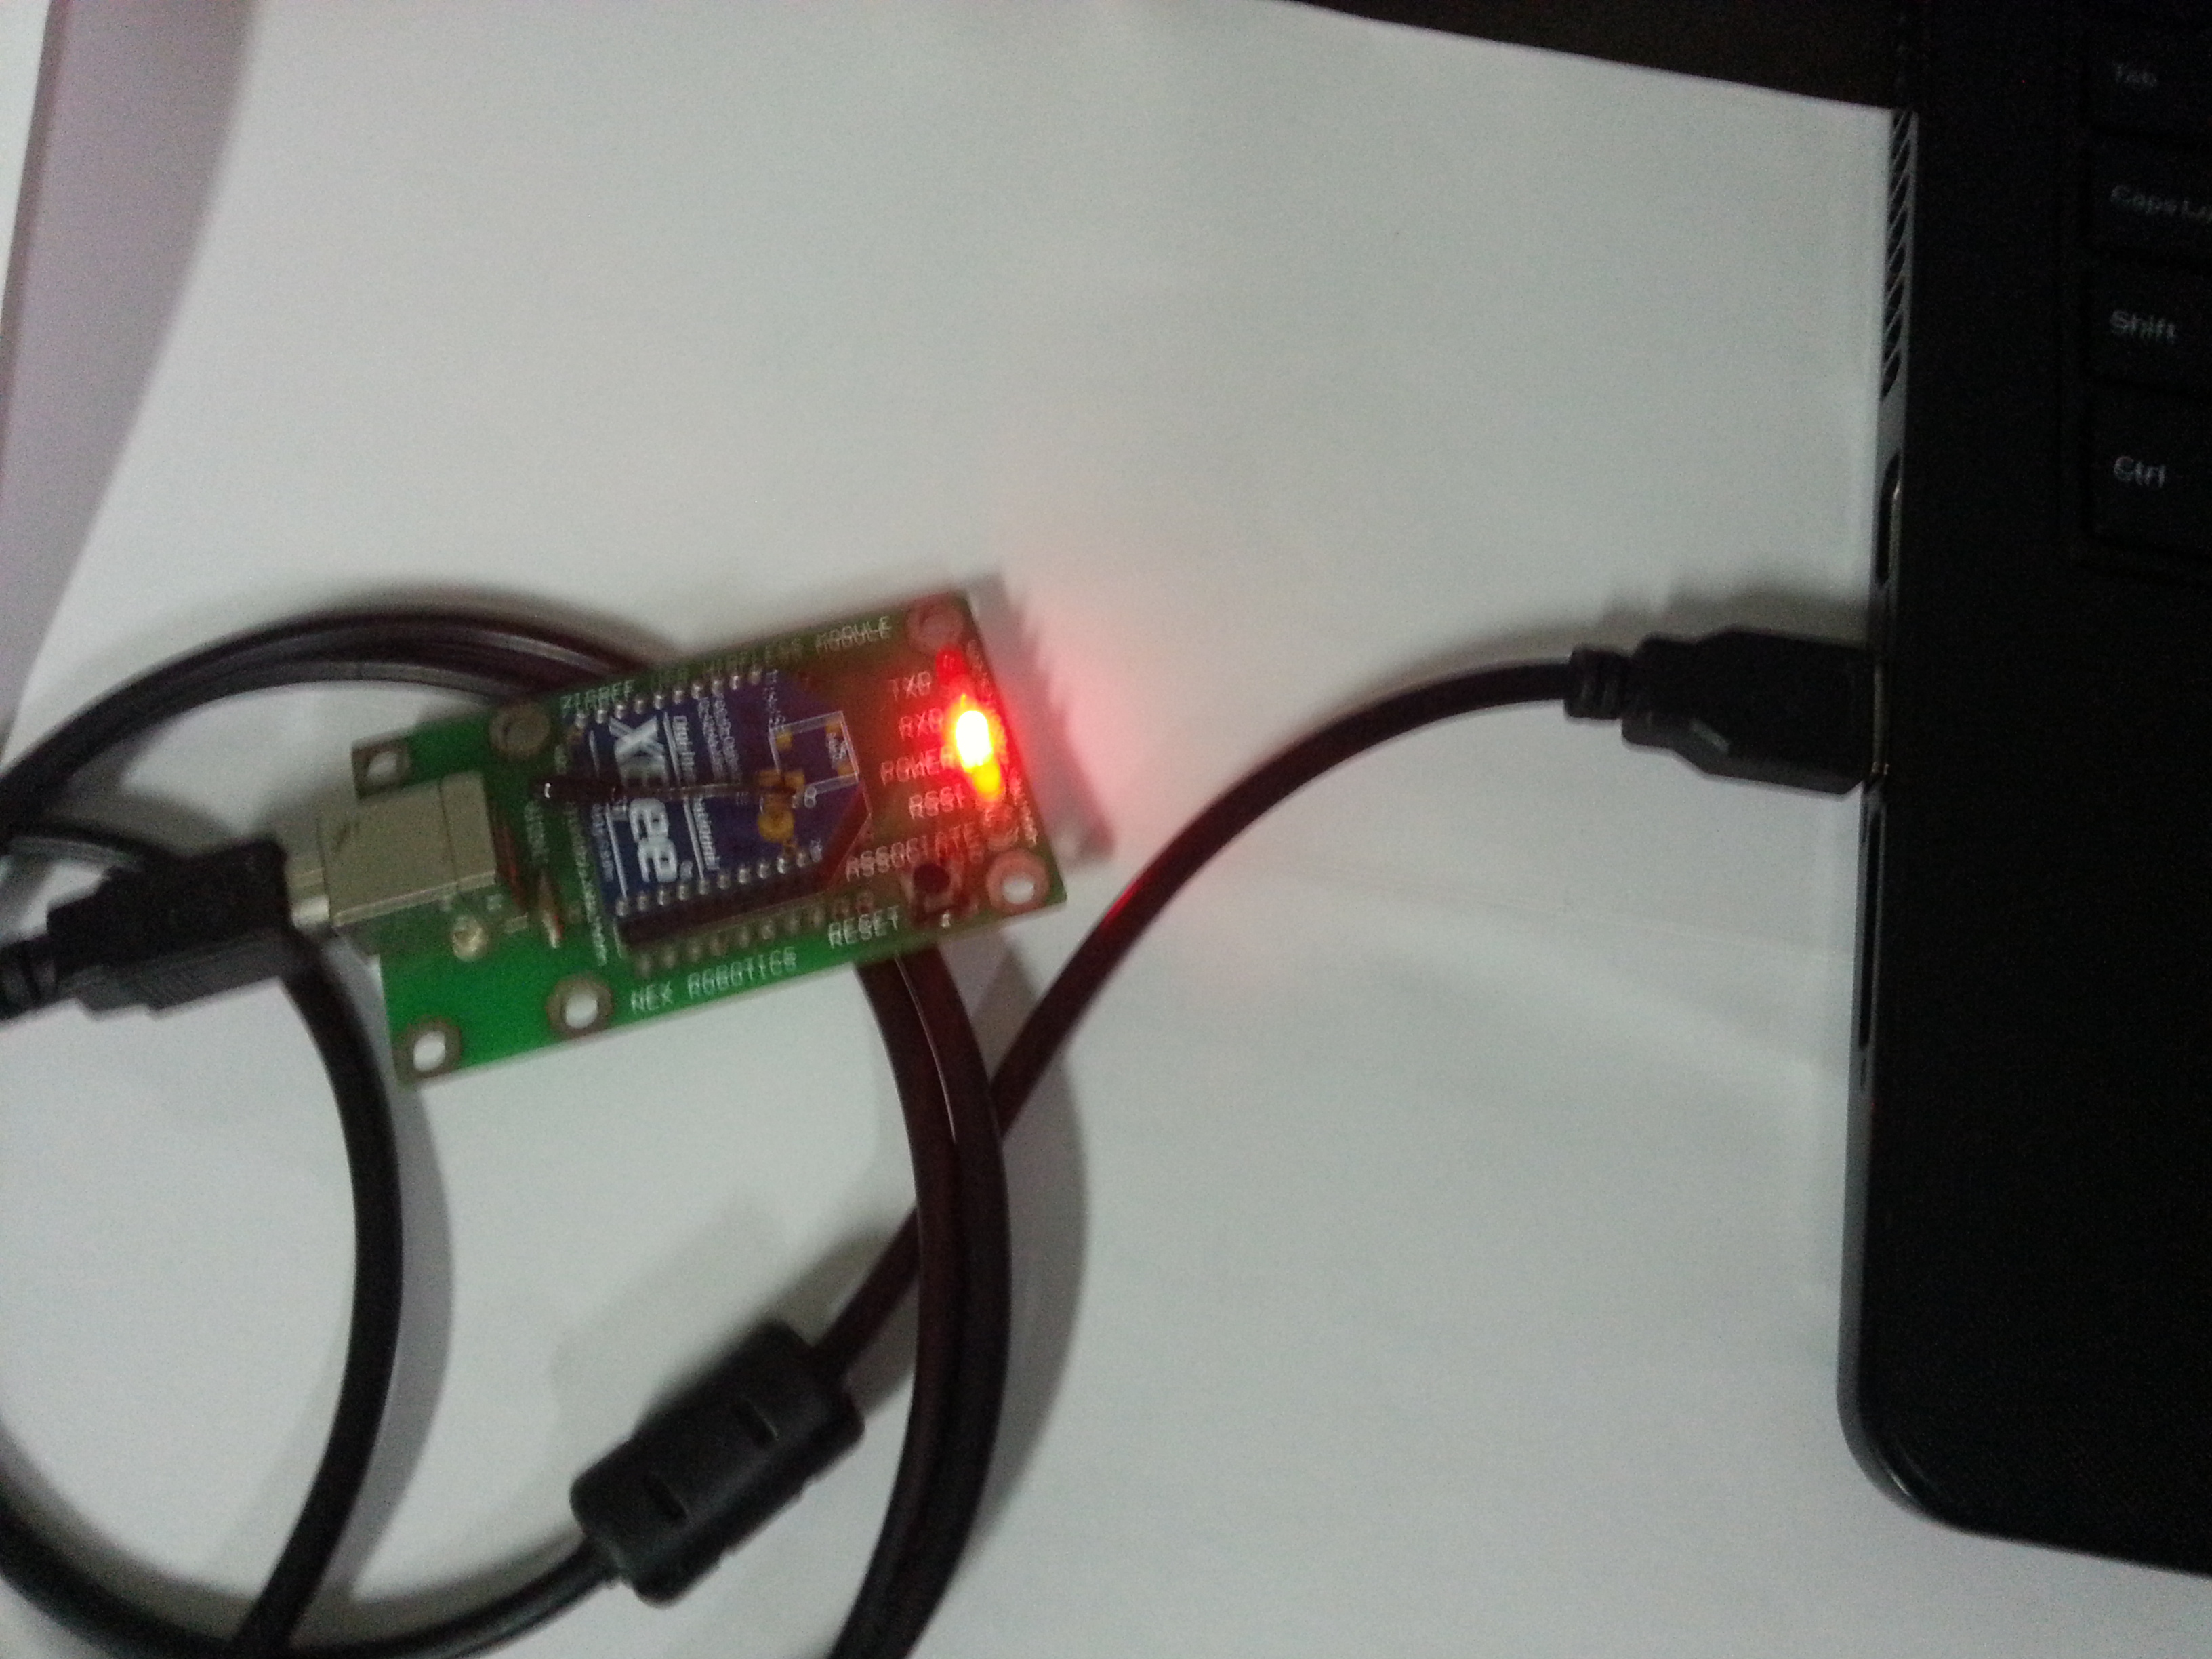
\includegraphics[scale=0.1]{20160722_194935.jpg}
	\end{figure}
	 
	 \item Turn ON bluetooth and run wiced.js file in terminal
	 
	 \begin{figure}[h]
    \centering
	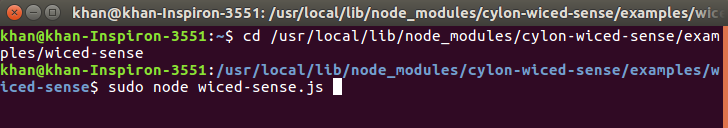
\includegraphics[scale=0.5]{runwicedjs.png}
	\end{figure}
	 
	 \newpage
	 \item Set temperature of which you need to be notified.
	 \begin{figure}[h]
    \centering
	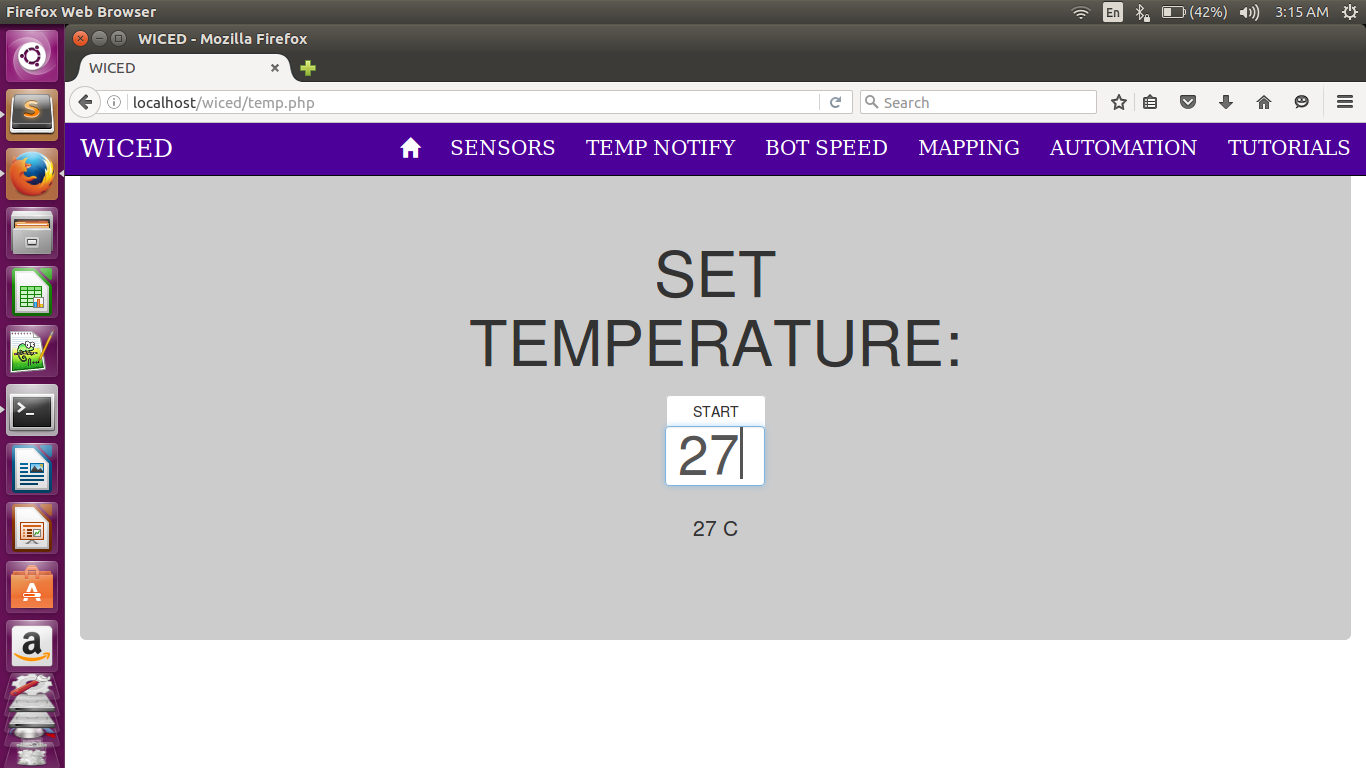
\includegraphics[scale=0.3]{temp12.png}
	\end{figure}
	 
	 \item Selected temperature will be displayed immediately at the bottom of form.
	  \item As th current temperature/Wiced sense temperature exceeds above fixed temperature , then a popup alert will appear to notify the user.
	 
	  \begin{figure}[h]
    \centering
	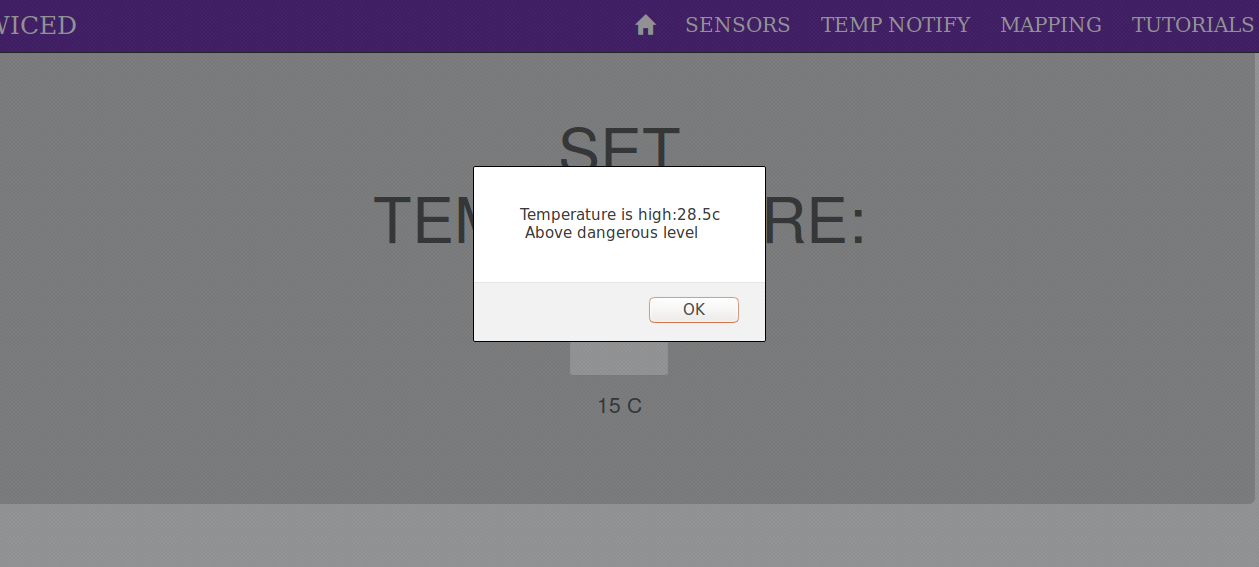
\includegraphics[scale=0.3]{popup_alert.png}
	\end{figure}
	 \end{itemize}
	 
	 
	 \newpage
	  \subsection{How to map the path of robot ?}
	 \begin{itemize}
	 \item Open terminal and start lampp local server.
	 
	 	\begin{figure}[h]
    \centering
	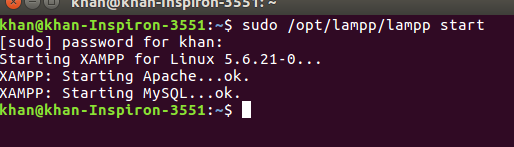
\includegraphics[scale=0.5]{lampstart.png}
	\end{figure}
	 
	 \item Open mapping.html page in website.
	 \item  Insert USB (zigbee) into the USB slot of local machine.
	  
	 \begin{figure}[h]
        \centering
	    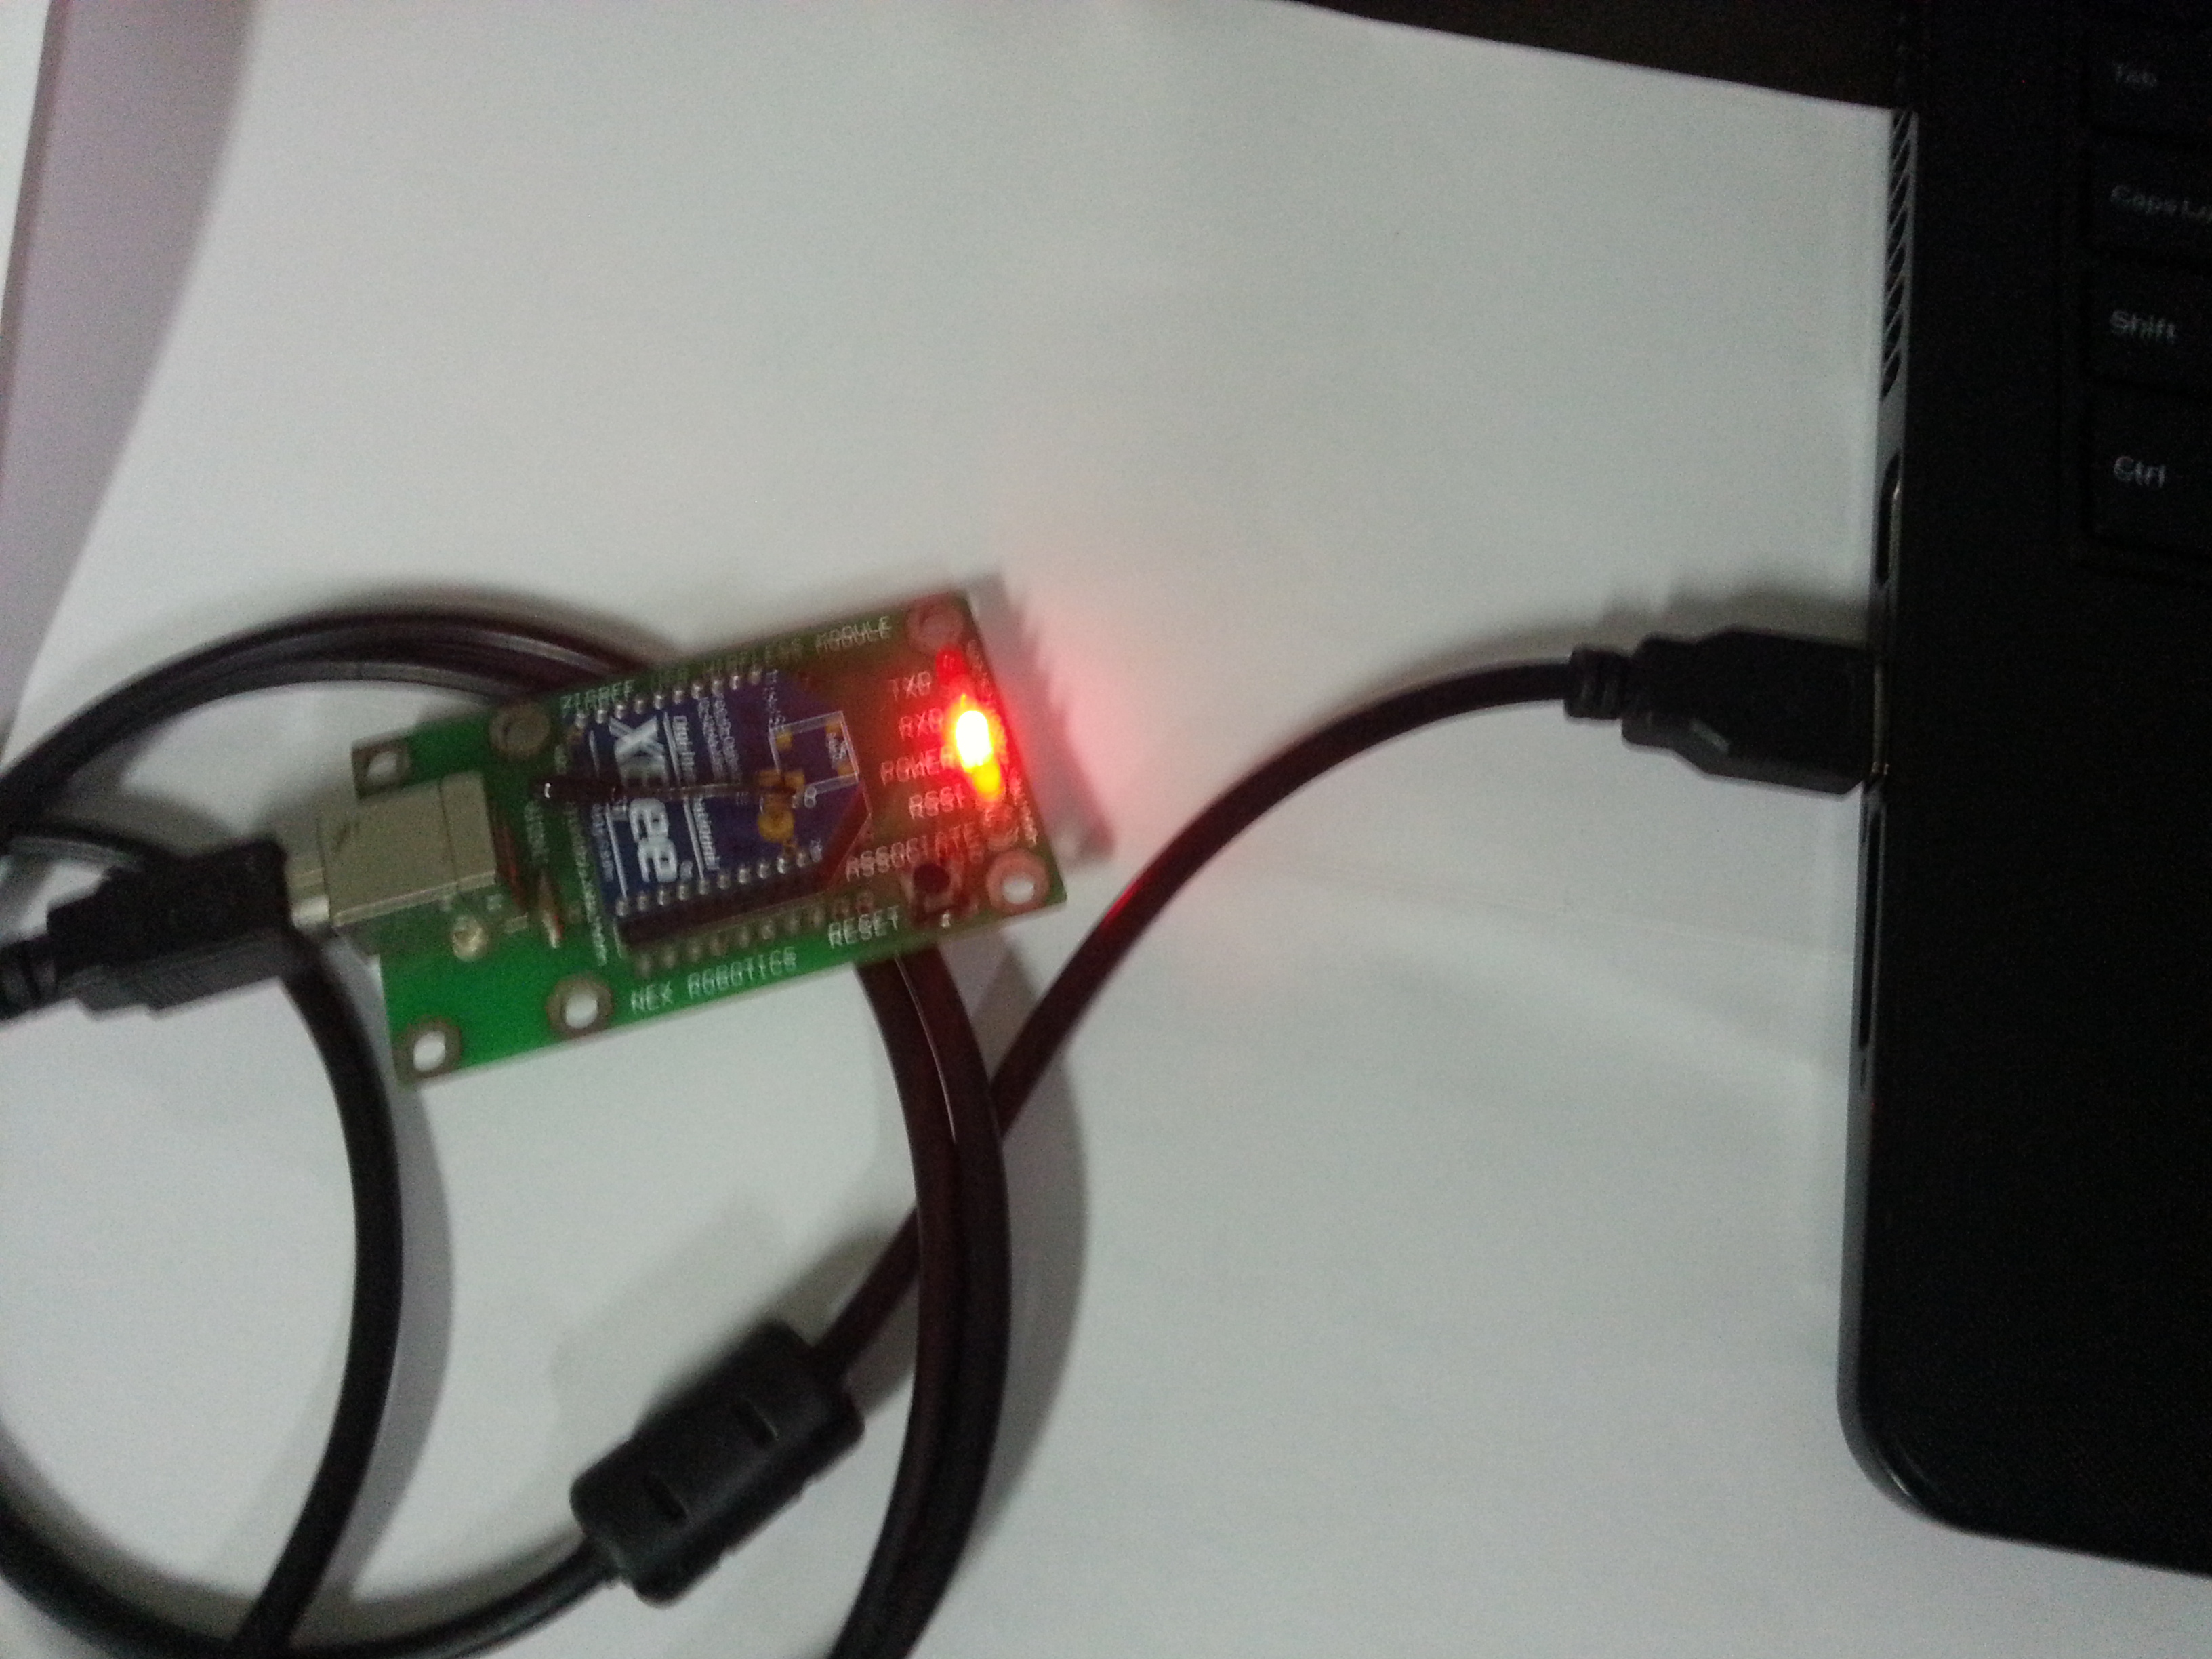
\includegraphics[scale=0.08]{20160722_194935.jpg}
	\end{figure}
	\item Place wiced sense on bot where keychane part of wiced must be facing forward .
	\begin{figure}[h]
    \centering
	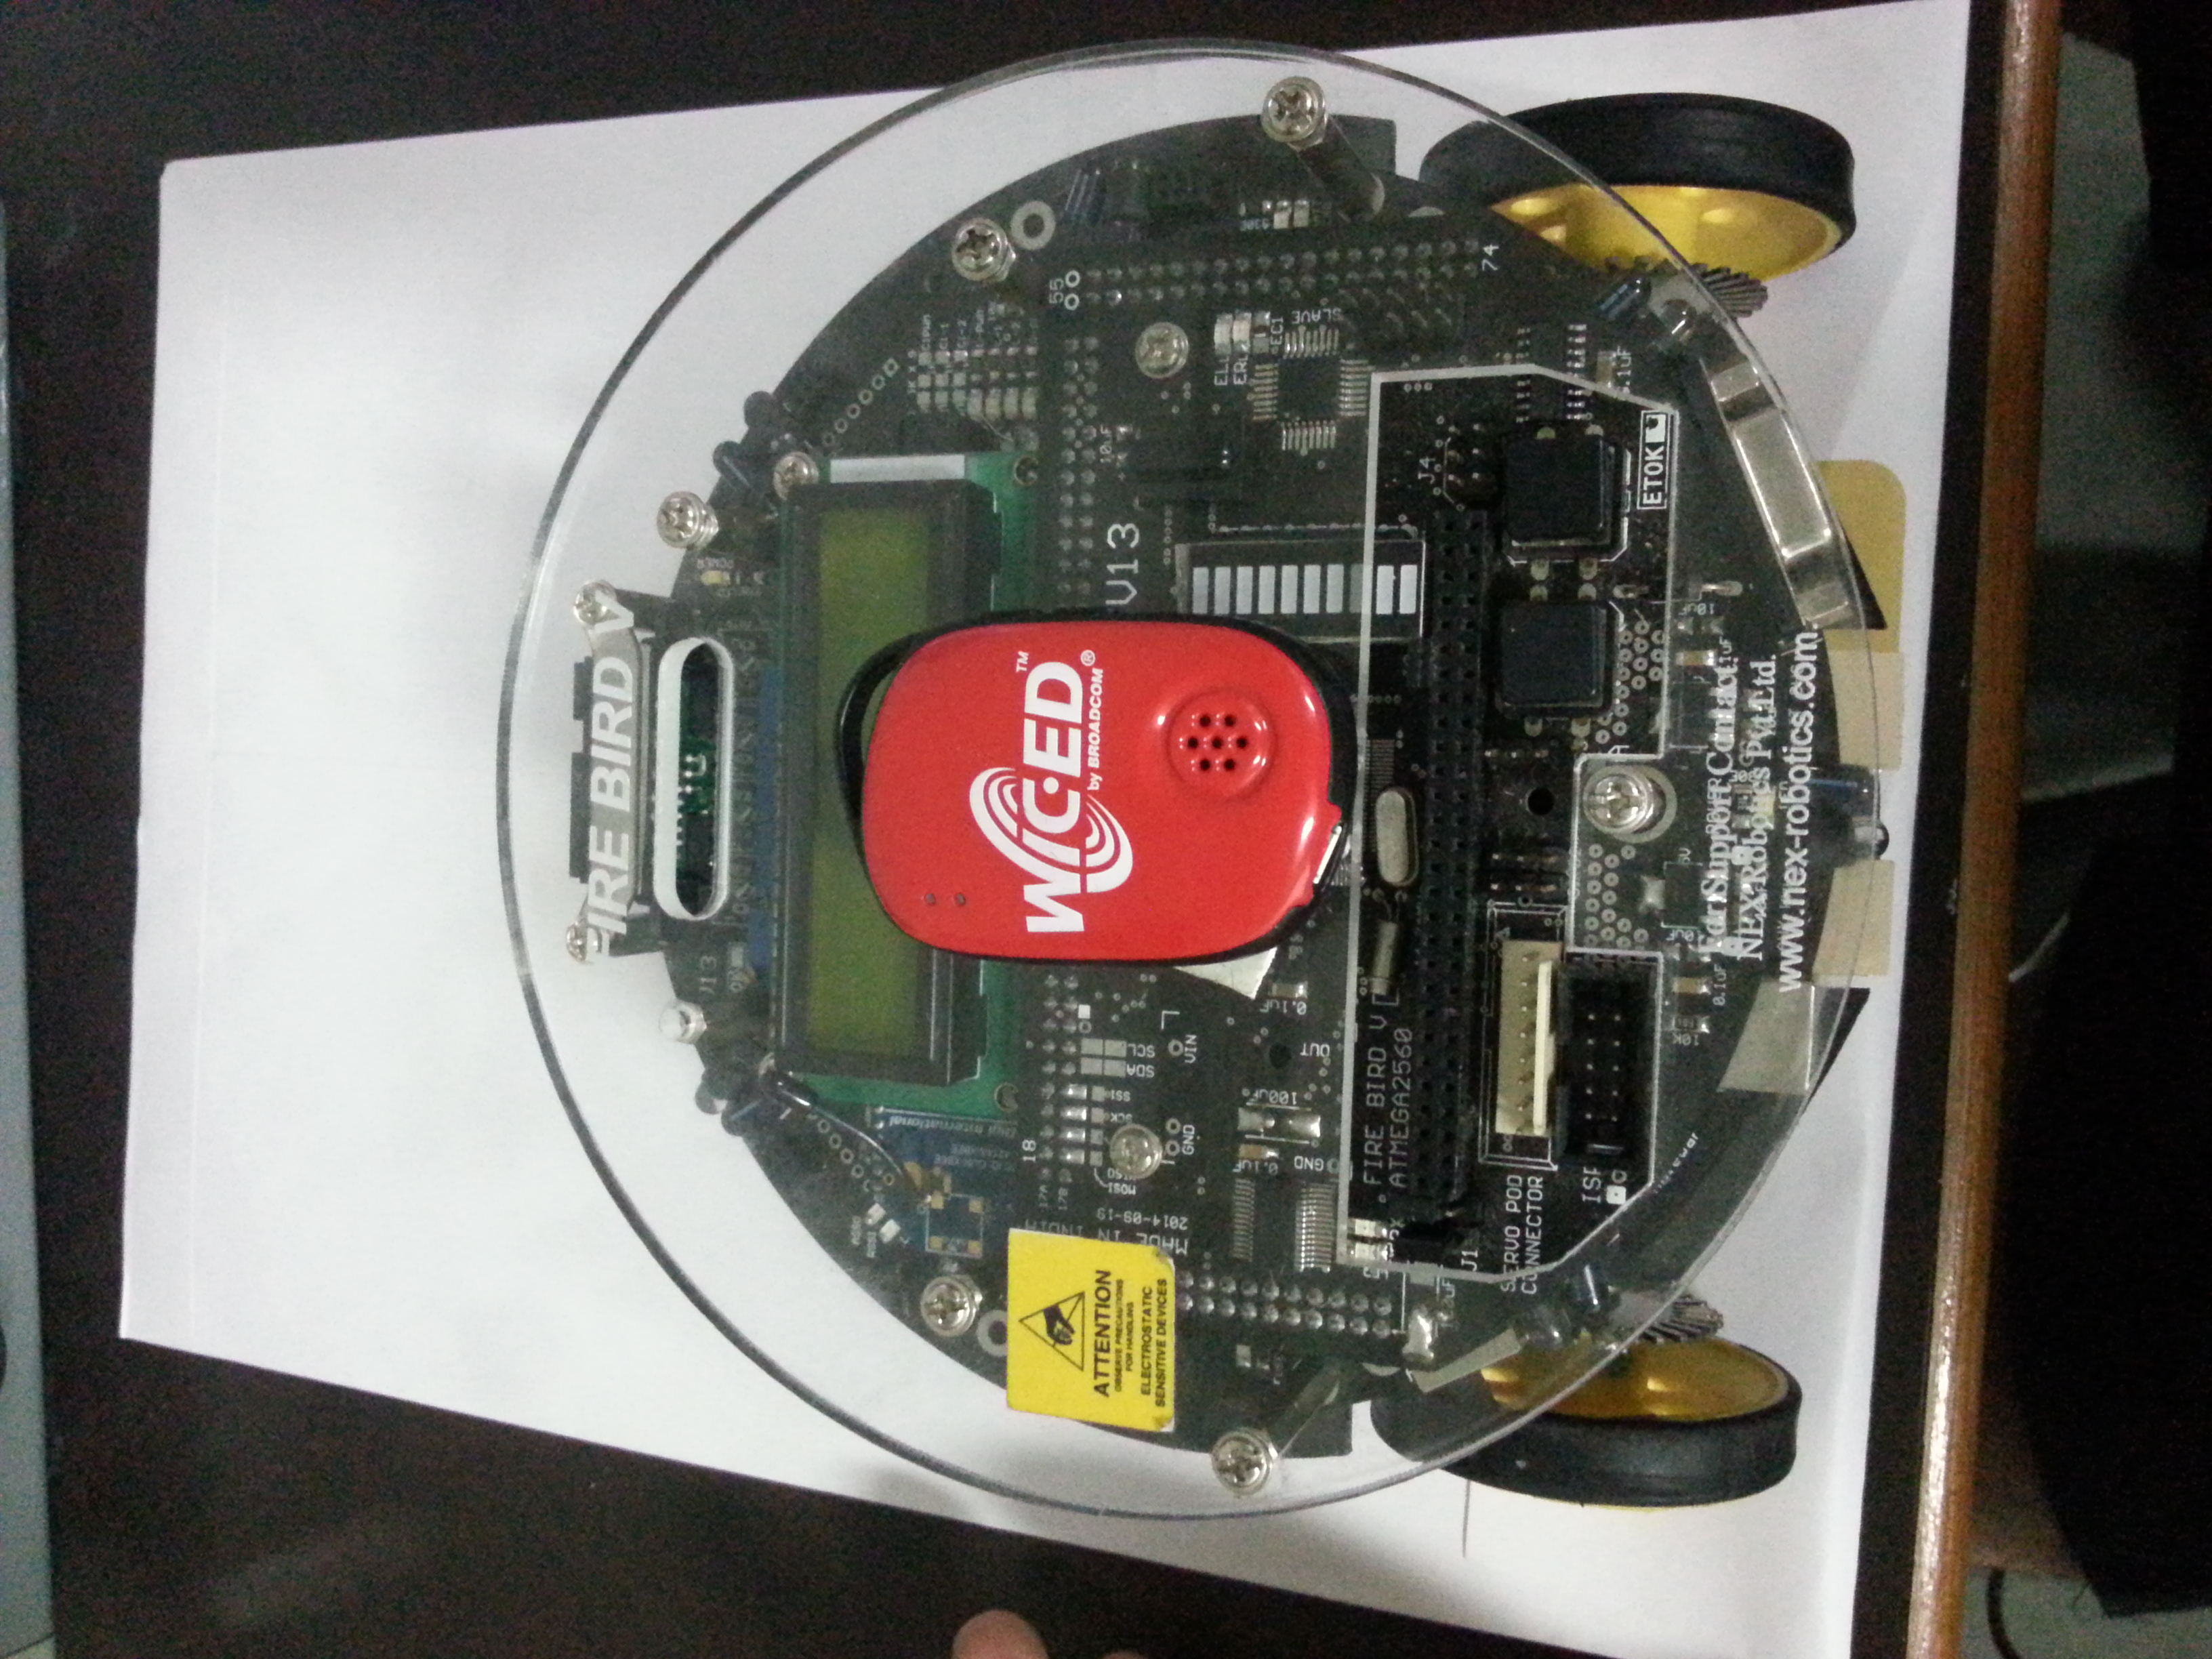
\includegraphics[scale=0.1]{20160722_195513.jpg}
	\end{figure}
	 \item Turn ON system bluetooth and keep the bot at the start position of the path or area to be mapped.
	 
	 
	 \newpage
	\item Turn WICED ON by pressing the app button.
	 \item Do not move the bot after placing at start position.
	 \item Run wiced-sense.js file and wait for data to arrive.
	 
	 	\begin{figure}[h]
    \centering
	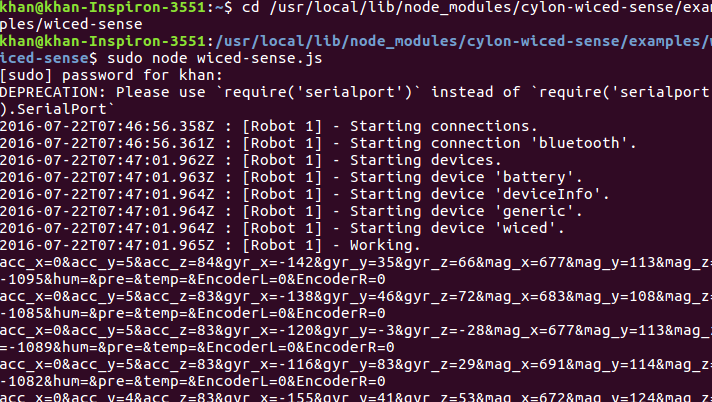
\includegraphics[scale=0.5]{data_arraives.png}
	\end{figure}
	
	\item AS the data arrives on terminal, immediately refresh mapping.html page.
	
	
		\begin{figure}[h]
    \centering
	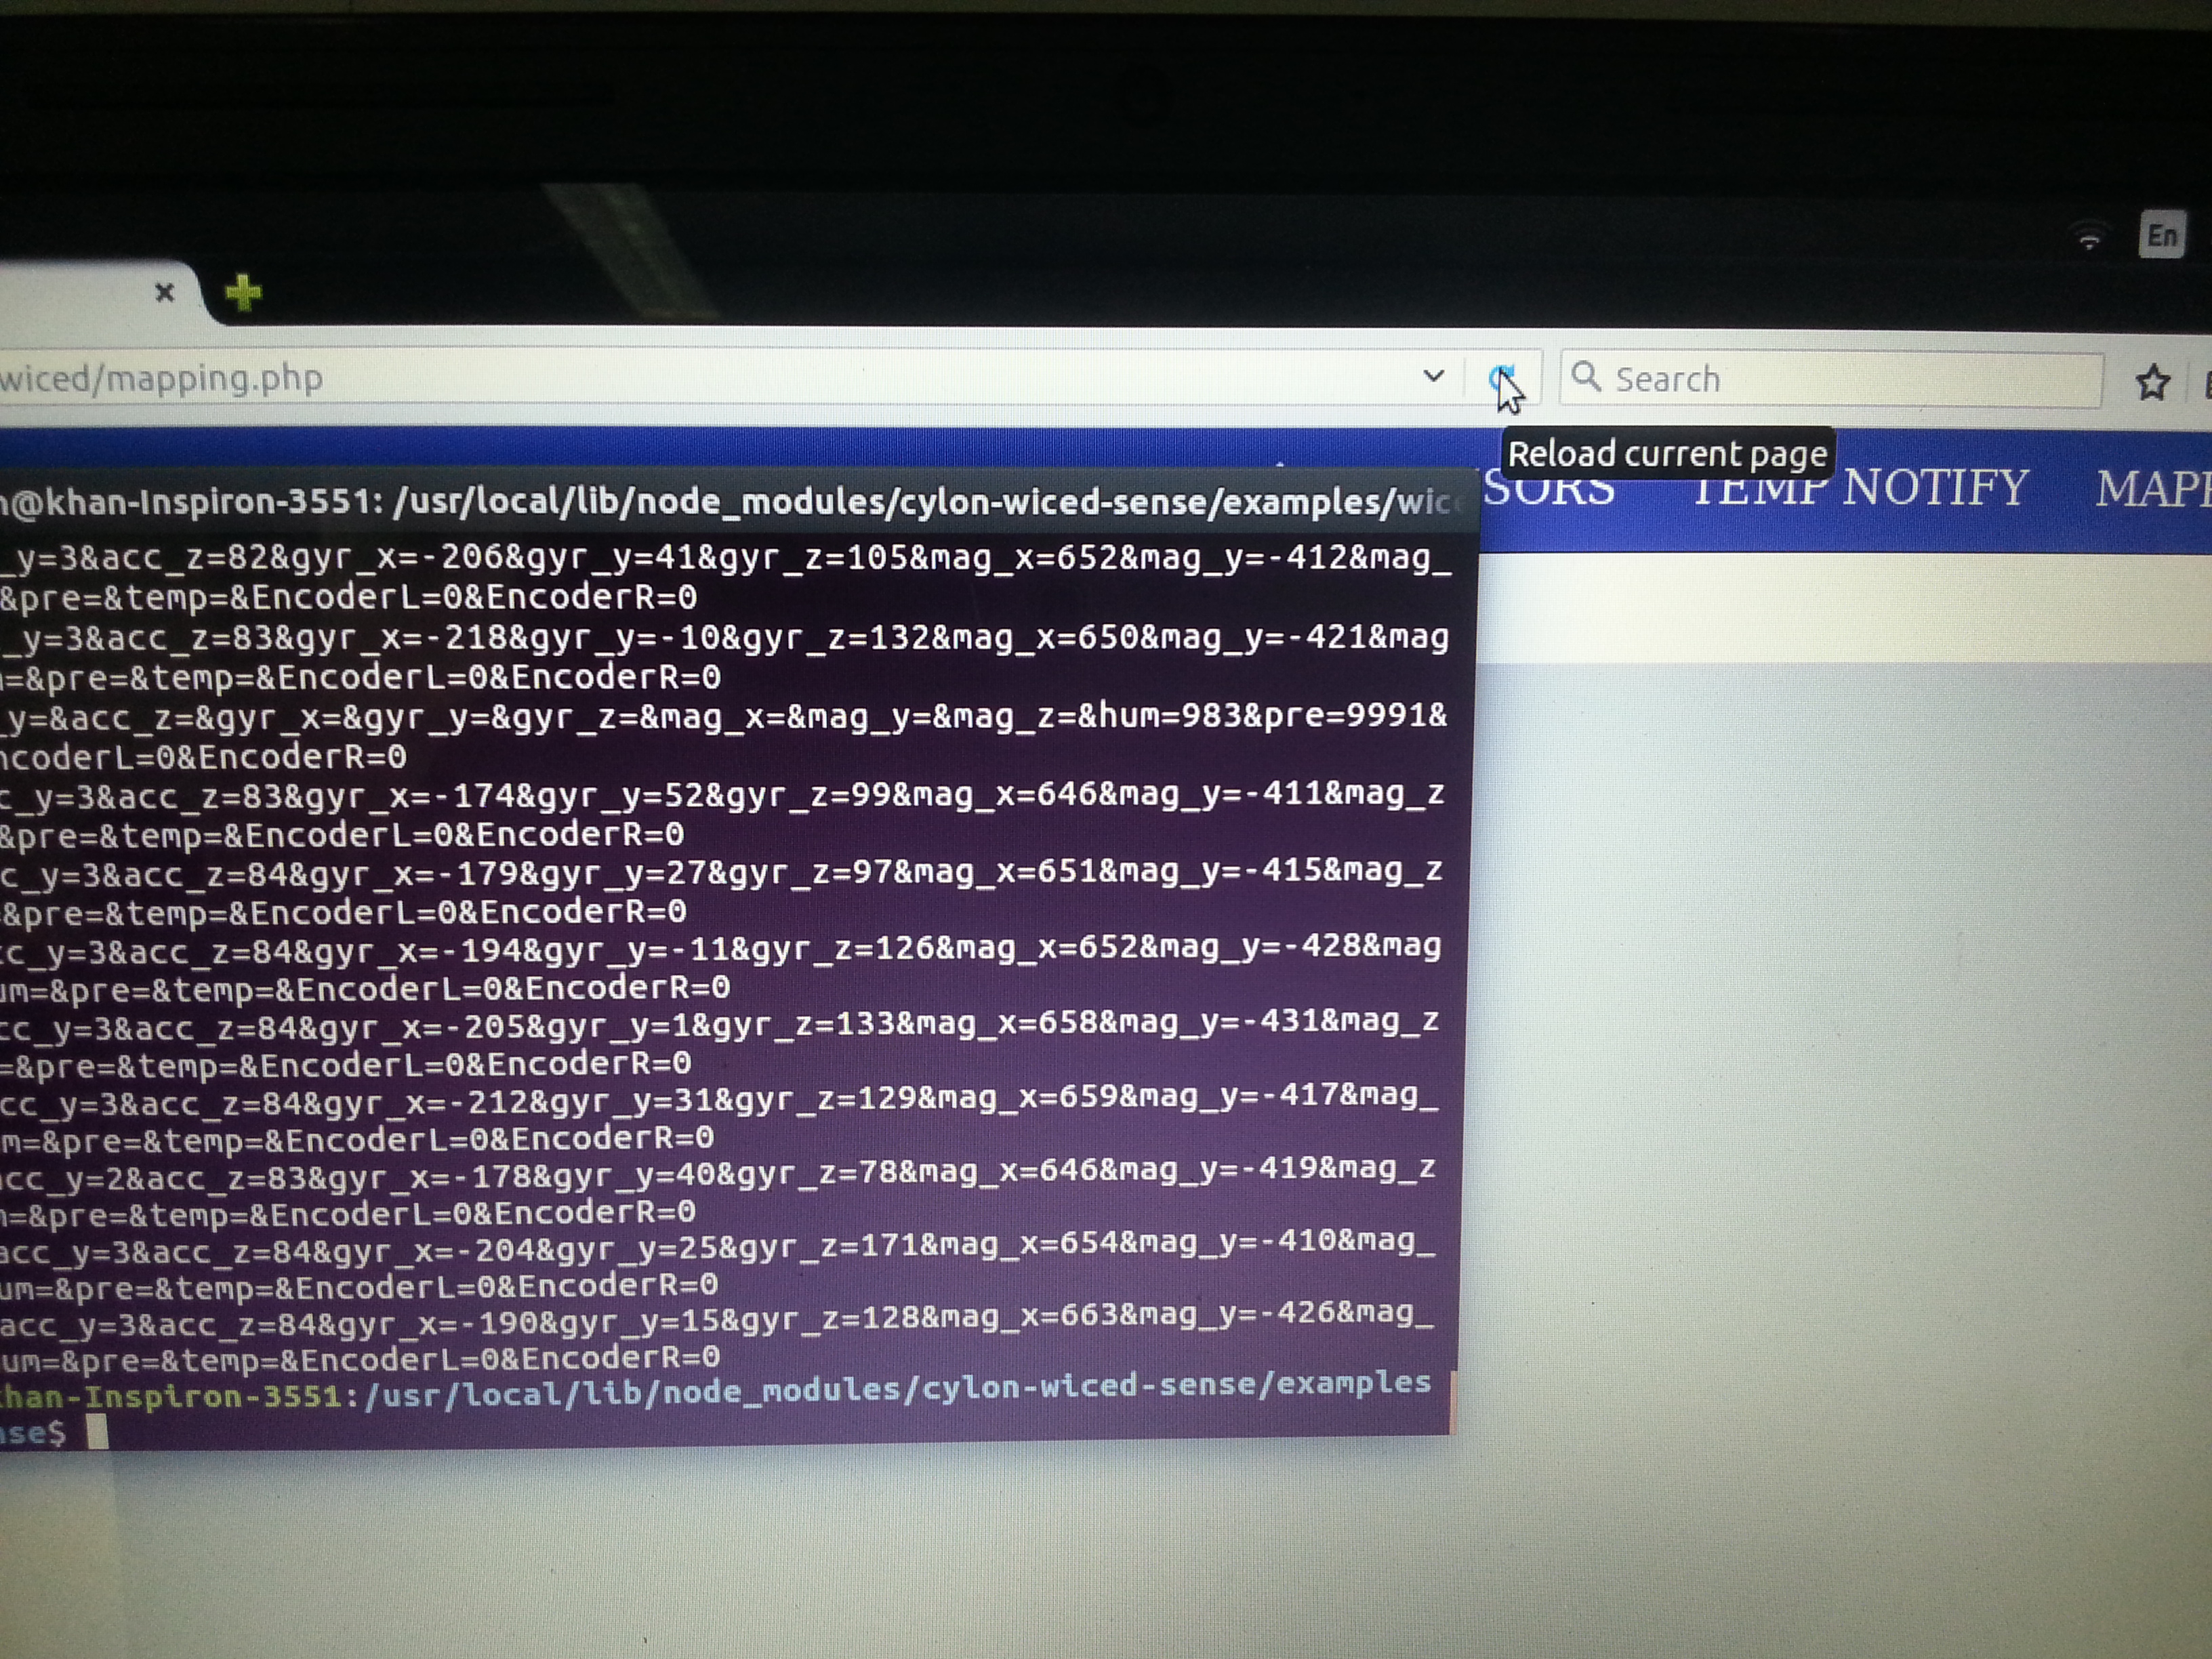
\includegraphics[scale=0.1]{20160722_195821.jpg}
	\end{figure}
	
	\newpage
	\item Turn on bot to move forward. As the bot moves , path is drawn accordingly.
	
	\item After mapping is done inorder to terminate the process enter Cltr+C in terminal. Hence process will be terminated
	 	 \end{itemize}


	\end{document}